\chapter{Uživatelské rozhraní}
Grafická uživatelská rozhraní (GUI) jsou klíčovým prvkem většiny aplikací. Jsou to první, co uživatel uvidí a co mu umožní s aplikací interagovat. Dobře navržené GUI může znamenat rozdíl mezi úspěchem a neúspěchem aplikace. Měl by být intuitivní, snadno ovladatelné a příjemné na pohled. V následující kapitola bude věnována základním principům designu GUI.

\section{Stručná historie GUI}
Počátek grafických rozhraní se datuje do osmdesátých let minulého století, kdy firma Xerox vyvinula počítač Alto. Jednalo se o první počítač, jehož rozhraní se skládalo z oken, ikon a používalo myš k ovládání. Toto grafické rozhraní pak posloužilo jako odrazový můstek a základ dalším projektům. Jeden z nich byl například Apple Macintosh, který grafické uživatelské rozhraní popularizoval. Dále přišel operační systém Windows, který GUI posunul ještě dál mezi mainstreamové uživatele. GUI se postupem let vyvíjelo společně s novými technologiemi a nyní je neoddělitelnou součástí téměř všech počítačových systémů.

\section{Zásady vývoje webového GUI}
Následující zásady jsou základem přívětivého UI, ve kterém se dokáže uživatel snadno orientovat a které je příjemné na pohled. Vychází z praktických zkušeností grafiků i psychologických studií.

\subsection{Vzhled stránky}
Následující text se věnuje několika základním principům, které by mělo moderní uživatelské rozhraní splňovat.\cite{principles_of_design}

\subsubsection*{Kontrast}
Kontrast je jedním z nejdůležitějších prvků designu. Zajišťuje, že text a další prvky jsou čitelné a viditelné. Je důležitý pro umocnění dojmu a pro zvýraznění důležitých prvků.

\subsubsection*{Balanc}
Všechny prvky na stránce mají pomyslou váhu, která je dána jejich velikostí, barvou, kontrastem a dalšími faktory. Zajišťuje, že tyto prvky jsou rozloženy tak, aby stránka působila vyváženě a přehledně.

\subsubsection*{Důraz}
Důraz slouží pro zvýraznění důležitých prvků a k pomyslnénu ukrytí těch méně podstatných. Můžeme tak ovládat výraznost jistých informací a zároveň usměrňovat pozornost uživatele.

\subsubsection*{Proporce}
Správně určené proporce podporují výše zmíněný balanc. Pomáhají uživateli orientovat se na stránce a zároveň zajišťují, že stránka působí přehledně a esteticky.

\subsubsection*{Hierarchie}
Hierarchie je v designu klíčová, zejména pokud jde o zdůraznění důležitých prvků. Tento princip je často demonstrován prostřednictvím titulů a nadpisů. Titul stránky by měl okamžitě vyniknout jako nejdůležitější prvek, zatímco nadpisy by měly být formátovány tak, aby naznačovaly svůj význam ve vztahu k sobě navzájem a k obsahu, který uvádějí.

\subsubsection*{Opakování}
Opakování je účinným nástrojem pro zdůraznění a sjednocení myšlenek v rámci designu. Lze ho dosáhnout konzistentním použitím barev, písem, tvarů nebo jiných prvků designu. Konzistentní formátování pomáhá sjednotit prvky na celé stránce.

\subsubsection*{Rytmus}
Slovem rytmus je myšlen styl, jakým jsou prvky (ať už mezery, barvy, velikosti, atd.) na stránce uspořádány a v jakém pořadí použity. Některé rytmické vzory mohou vzbuzovat pocit uspořádanosti a přehlednosti, zatímco jiné mohou působit chaoticky.

\subsubsection*{Vzor}
V uživateli vzory vyvolávají pocit předvídatelnosti a pohodlí. Může se jednat například o rozložení stránky, které se běžně používá, nebo o způsob zadávání dat, který je uživatelům známý.

\subsubsection*{Volný prostor}
Volný prostor (white space) je prázdný prostor mezi prvky na stránce, který pomáhá zvýraznit důležité prvky a zároveň zajišťuje, že stránka není přeplněná.

\subsubsection*{Pohyb zraku po stránce}
Tohoto principu lze dosáhnout dodržením výše zmíněných prvků. Jde o kombinaci všech předešlých principů a jejich aplikaci tak, aby uživatel mohl snadno a pohodlně stránku použít.

\subsubsection*{Rozmanitost}
Na rozdíl od předešlých bodů, rozmanitost nenapomáhá orientaci na stránce, ale zajišťuje, aby byla pro uživatele zajímavá.

\subsubsection*{Spojitost}
Spojitost zajišťuje, že všechny prvky na stránce působí jako celek. Většinou se jedná o opakování barev, či používání minimálního množství fontů.

\subsubsection{Teorie barev}
Výběr barev je nedílnou součástí vývoje každého GUI. Teorie barev se zabývá vztahy mezi barvami a jejich významem. Poznáním těchto nuancí může vývojář využít barvy k ovlivnění uživatelova vnímání své aplikace. Různé barvy mohou budit různý psychologický a emocioální význam. Teorie barev poskytuje základní pravidla a směrnice pro efektivní použití barev v designu, aby se dosáhlo esteticky příjemného výsledku a vyvolalo se požadované emoční nebo vizuální působení. Teorie barev také udává, že existuje několik kategorií základních barev:
\begin{itemize}
    \item \textbf{Primární barvy}: Červená, modrá a žlutá. Tyto barvy nelze vytvořit kombinací jiných barev.
    \item \textbf{Sekundární barvy}: Zelená, fialová a oranžová. Tyto barvy vzniknou smícháním dvou primárních barev.
    \item \textbf{Terciární barvy}: Těchto šest barev vznikne smícháním primárních a sekundárních barvev. Patří sem například růžová, tyrkysová, či žlutozelená.
\end{itemize}

Těchto dvanáct barev samozřejmě není jedinými barvami, které lze zejména v počítačové grafice použít. Díky tomu se začalo v grafice používat takzvaný color wheel (barevný kruh).\cite{color_theory_design}

\subsubsection*{Color wheel}
Barevný kruh se často používá díky jeho intuitivnímu rozložení barev. Obsahuje všechny barvy, které lze vytvořit smícháním tří primárních barev a díky přidání černé, či bílé barvy umožňuje i úpravu jejich odstínů. Existuje několik způsobů, jak za pomoci tohoto kruhu vybrat (některé z nich můžeme vidět na obrázku \ref*{fig:color_theory}):\cite{color_wheel,color_schemes}
\begin{itemize}
    \item \textbf{Komplementární}: Barvy, které jsou na opačných stranách kruhu. Při jejich kombinaci vzniká kontrastní efekt.
    \item \textbf{Monochromatické}: Jedná se o sadu odstínů jedné barvy. Vytváří harmonický efekt.
    \item \textbf{Analogické}: Barvy, které jsou vedle sebe na kruhu. Vytváří přirozený a pohodlný efekt, ale je vhodné vybrat jednu z barev jako hlavní a zbytek používat pouze jako akcenty.
    \item \textbf{Triadické}: Kombinace tří barev, které na kruhu tvoří rovnostranný trojúhelník. Podobně jako způsob komplementární, také vytváří kontrastní efekt.
    \item \textbf{Rozštěpená komplementární}: Variace komplementární kombinace, kde se namísto protější barvy, používají barvy s ní sousedící. 
    \item \textbf{Tetradické}: Čtyři barvy, kde vždy dvě z nich tvoří komplementární pár -- na barevném kruhu vytváří obdélník. Vytváří kontrastní efekt, ale zároveň je možné vytvořit i harmonický efekt, pokud se barvy správně kombinují.
\end{itemize}

\begin{figure}[H]
    \centering
    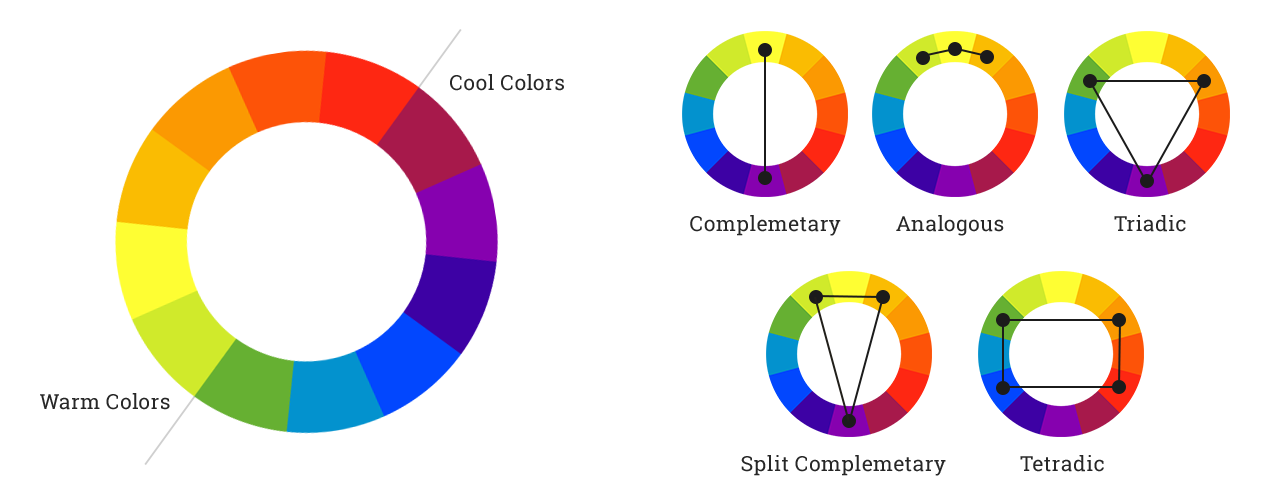
\includegraphics[width=0.9\textwidth]{resources/figures/color_theory.png}
    \caption{Barevné kolo a dělení barev.\cite{color_schemes}}
    \label{fig:color_theory}
\end{figure}

Dále se barvy dělí na teplé a studené. Teplé barvy jsou červené, oranžové a žluté části spektra a často evokují radost a energii. Studené barvy jsou zelené, modré a fialové části spektra a často evokují klid a harmonii. Výběr teplých, či studených barev může mít vliv na celkový dojem, který uživatel z aplikace získá.\cite{color_theory_design} 

\subsubsection{Typografie}
Typografie je umění používání písma a fontů k tomu, aby byl text čitelný, srozumitelný a příjemný ke čtení. Hraje klíčovou roli v designu UI tím, že ovlivňuje rozpoznatelnost značky, rozhodování a pozornost uživatele. Dobrá typografie pomáhá při předávání informací a integruje se s ostatními prvky rozhraní, zlepšujíc celkovou vizuální rovnováhu a uživatelskou zkušenost.\cite{typography}

\subsection{Použitelnost}
Úzce souvisí se vzhledem stránky a často se tato témata překrývají, ale zároveň je to samostatný princip, který je nutno uvést zvlášť. Zahrnuje všechny aspekty, které napomáhají uživateli k snadnějšímu a pohodlnějšímu užívání stránky. Zahrnuje například:\cite{principles_of_ui_design}

\subsubsection*{Konzistence}
Konzistence je klíčová pro uživatelskou přívětivost. Uživatelé se rychleji naučí, jak stránka funguje, pokud je konzistentní. To znamená, že by vývojář měl dodržovat stejné rozložení a navigaci mezi jednotlivými stránkami.

\subsubsection*{Zkratky}
Zkratky mohou urychlit a tím zpříjemnit uživatelův pohyb po stránce. Využitím odkazů v menu, či přesměrování díky kliknutí na logo můžeme tohoto výsledku dosáhnout. Takovéto oskaty by měly být intuitivní a logické.

\subsubsection*{Zpětná vazba}
Zpětná vazba je důležitá pro uživatele, aby věděl, zda se akce, kterou chtěl provést, povedla, či nikoliv, či jestli je možnost na nějaký prvek stránky kliknout. Tohoto můžeme dosáhnout pomocí animací, změny barvy, či zvýrazněním.

\subsubsection*{Uzavření dialogu}
Uzavření dialogu je důležité pro uživatele, aby věděl, že jeho akce byla úspěšná a může přejít k dalšímu kroku. Tohoto můžeme dosáhnout například přesměrováním na jinou stránku, či zobrazením dialogu, který uživateli potvrdí, že jeho akce byla úspěšná.
\pagebreak

\subsubsection*{Prevence chyb}
Zabezpečení proti nesprávným vstupům z uživatelovy strany je podstatná pro předejití zbytečných chyb, které by mohly vést k frustraci. Toho můžeme dosáhnout například tím, že nebudeme uživateli dovolovat zadávat písmena do pole, které by mělo obsahovat pouze čísla. Pokud už chyba nenávratně nastane, je důležité uživatele informovat o tom, co se stalo a jak ji může napravit.

\subsubsection*{Možnost vrácení}
Pokud se uživatel rozmyslí, či udělá chybu, měl by mít možnost svou akci jednoduše zrušit a vrátit se do předešlého stavu stránky.

\subsubsection*{Locus of control}
Tento fenomén by se dal volně přeložit jako těžiště řízení. Uživatelé chtějí mít pocit, že aplikaci řídí a že rozhraní reaguje na jejich akce. Takového pocitu můžeme mimo jiné dosáhnout tím, že se zeptáme na potvrzení nějaké akce, například odchodu ze stránky s neuloženými daty. Tím uživateli dáme pocit větší kontroly.

\subsubsection*{Minimalizace nároků na uživatele}
Klíčová zásada pro uživatelské rozhraní je minimalizace kognitivní zátěže. Kognitivní zátěž může snížit uživatelovu schopnost vykonávat důležité úkoly, proto je kritické, aby počítače převzaly co nejvíce úkonů na sebe. Uživateli můžeme vypomoci třeba zapamatováním si jeho přihlašovacích, či osobních údajů. aby je nemusel zadávat při každém přihlášení. Při návrhu bychom měli vždy dávat přednost rozpoznání před vzpomínáním, abychom uživatelům umožnili rychle a bez problémů dokončit své úkoly.

\subsubsection{Responzivnost}
Jedna z nejdůležitějších vlastností moderního GUI. Responzivní design zajišťuje, že stránka bude vypadat dobře na všech zařízeních, od mobilních telefonů až po stolní počítače a to pomocí změny velikosti, schování, či přesunutí prvků na stránce. K tomu se využívají vlastnosti jazyka CSS, nejčastěji media queries, které umožňují nastavit různé styly pro různé velikosti obrazovek. Responzivní design je v dnešní době kriticky potřebný, protože většina uživatelů používá k prohlížení internetu mobilní zařízení a je důležité, aby se jim stránka zobrazila správně a byla snadno použitelná.\cite{responsive_design}

\section{GUI ve vybraných hybridních hrách}
Tato sekce se bude věnovat analýze uživatelského rozhraní několika vybraných hybridních her. Jedná se o hry, které jsou v současné době populární a mají velkou základnu hráčů. Analýza bude zahrnovat vzhled a funkce GUI, které hra poskytuje.

\subsection{Na vlnách neznáma}
Tato aplikace je vyvíjena a udržována společností Plaid Hat Games, která vydala i samotnou hru. Jde o oficiální rozšíření a hlavní způsob, jak hru hrát. Společnost později vydala i pdf, které do určité míry tuto aplikaci nahrazuje, ale hráčům poskytuje méně možností. Jedná se o webovou aplikaci, kterou je možné stáhnout a používat offline, avšak bez některých funkcionalit, jako jsou například rozšíření, či audio nahrávky.

\subsubsection{UI}
Kompaktní vzhled aplikace napovídá, že byla primárně určena pro mobilní zařízení -- je tedy i bez velkých změn velmi dobře použitelná pro počítače. Jedná se o jednostránkovou aplikaci s jednoduchým a přímočarým designem. Při spuštění vás přivítá logo hry a přívětivá a barevná grafika, která odpovídá fantasknímu námořnímu stylu hry. Samotná stránka obsahuje jen několik tlačítek; začít hrát, nastavení, ke stažení, varianty hry a o aplikaci. Celá aplikace je přeložena do několika jazyků, a to včetně češtiny.

\subsubsection{Funkce}
Při spuštění hry se zobrazí výběr příběhové linky, kterou chtějí uživatelé zažít. Po vybrání se zobrazí stránka s textovým polem, do něhož hráči mohou zadat číslo záznamu, který chtějí zobrazit. Toto číslo je jim oznámeno v předešlém záznamu, či v knize lokací a závisí na jejich dosavadních rozhodnutích. Dále je na stránce možnost zobrazit, jak mají hráči připravit herní plochu, statistiky jejich lodi a karty. Na stránce je také možnost zapnutí odpočtu, pokud se hráči rozhodují moc dlouho, či náhled historie zobrazených záznamů.

Aplikace slouží převážně k zobrazování výše zmíněných záznamů a k podporování imerze přehráváním ambientních zvuků a audionahrávek s narací příběhu. Mimo jiné také napomáhá s událostmi ve hře, jako například boji tím, že za pomoci uživatelových vstupů kontroluje statistiky nepřátel.
\pagebreak

\subsection{Gloomhaven Secretariat}
Aplikace Gloomhaven Secretariat je fanouškovskou aplikací, která vychází z nyní již zrušené aplikace Gloomhaven Helper. Jedná se o jednostránkovou webovou aplikaci sestavenou v Angularu. Jedná se o open-source software, na kterém se podílí množství fanoušků Gloomhavenu a je stále ve vývoji.\cite{gloomhaven_secretariat_github}

\subsubsection{UI}
Aplikace je určena pro desktop, či jiná zařízení s velkou obrazovkou. Je sice použitelná i na mobilních zařízeních, ale jedná se pouze o zmenšenou verzi klasické stránky bez dalších úprav, což znamená, že některá tlačítka jsou příliš malá pro pohodlné používání. Obsah se také zdá být poměrné jednoduchý, avšak už není tak intuitivní, jako u předešlého příkladu. Vzhled UI, je příjemně a čistě vypadající a navíc tematicky věrný samotné hře. Navigace po základní stránce je poměrně přímočará, avšak to samé už se nedá říct o rozsáhlých menu, které se skrývají téměř pod každým tlačítkem. Ty se mohou zdát na první pohled nepřehledné a u velké části z nich je nedostatek popisků, či vysvětlení, jak vlastně jednotlivá tlačítka fungují. Uživatel si tak musí nejprve odzkoušet, co vše je možné, což může být zdlouhavé a frustrující. Zároveň bych však chtěl podotknout, že aplikace má tlačítko zpět, kterým může uživatel vrátit opravdu jakoukoliv akci, takže pokud hráč udělá nějakou chybu, je snadné ji opět napravit. Obdobně je zde i tlačítko vpřed. Stránka také potřebuje neustálé vstupy od uživatele, aby dokázala správně plnit svou funkci, ty jsou však také někdy neintuitivní a jejich zadávání často zdlouhavé a repetitivní.

\subsubsection{Funkce}
Hned na úvodní stránce dostane uživatel možnost výběru příběhové linie, kterou chce začít a následně ho stránka vyzve k přidání postav. Dále je možnost přidat nepřátele postupně, či spustit takzvaný scénář, což je v pravidlech popsaná kombinace nepřátel, kteří se vyskytují v určité části příběhu. Při boji aplikace zobrazuje statistiky postav a nepřátel, jejich aktuální stavy a efekty a umožňuje je hráči kontrolovat a upravovat. Stránka také sama náhodně vybírá z možností nepřátelských akcí a umožňuje hráčům za monstra "táhnout karty" a tím udávat sílu a efekt těchto akcí. Další možnosti aplikace zahrnují vedení globálních statistik skupiny, jejich úspěšnosti, odemčených lokací a dalších věcí. Zároveň umožňuje ukládání a stahování dat několika započatých her najednou.

Nutno říci, že aplikace je skutečně multifunkční a nabízí hráčům velké množství automatizace a ukládání dat. Tím velmi ulehčuje hru, zkracuje čas její přípravy a zároveň zabraňuje chybám, které by mohly vzniknout při ručním vedení statistik.
\pagebreak

\section{Volba technologií pro vývoj GUI}
Zprvopočátku jsem vytvořil prototyp GUI v čistém HTML a CSS, abych věděl, jak bude samotný produkt zhruba vypadat. Poté jsem svou pozornost obrátil na výběr technologií, které budu pro vývoj GUI používat. Hlavními kandidáty byly frameworky React, Angular a Svelte.

\subsection{Frameworky}

\subsubsection{React}
React je jednou z nejpopulárnějších moderních platforem pro tvorbu webových aplikací. Je to open-source JavaScript knihovna vyvinutá a udržovaná společností Meta (bývalý Facebook). Používá deklarativní programovací paradigma, což znamená, že vývojář specifikuje, jak by měl výsledek vypadat, bez toho, aby musel explicitně popsat, jak daného výsledku dosáhnout. Zároveň je založen na komponentovém přístupu -- celý kód je rozdělen do menších celků zvaných komponenty, což je kombinace JS a HTML, které jsou modulární a znovupoužitelné. Díky jeho schopnosti aktualizovat jednotlivé komponenty se nejčastěji používá pro vývoj jednostránkových webových aplikací. React je známý svou komunitou a ekosystémem, který je kolem něj postavený. Díky tomu je možné najít spoustu předpřipravených komponent a knihoven, které urychlí vývoj aplikace. Zároveň má však poměrně strmou křivku učení, což z něj dělá nepřívětivou volbu pro začátečníky.

React využívá virtuální DOM, který zajišťuje rychlejší a efektivnější vykreslování změn. Při změně v komponentě se nevykreslí celá stránka, ale pouze upravená část. Tím se značně zrychlí vykreslování a zároveň sníží nároky na výkon.\cite{react, what_react_is_and_why_it_matters,angular_vs_react}

\subsubsection{Angular}
Angular je další z vysoce populárních frameworků pro vývoj UI. Opět se jedná o open-source platformu, nyní však vyvinutou a udržovanou společností Google. Angular je založen na jazyce TypeScript a stejně jako React využívá komponentového přístupu a deklarativního programovacího paradigmatu. Jeho převážný význam spočívá ve vytváření rozsáhlých dynamických webových aplikací. Na rozdíl od Reactu se jedná o plněhodnotný framework, který používá reálný DOM. Samotný framework je robustní a bezpečný, což z něj dělá ideální volbu pro vývoj aplikací, které pracují s citlivými daty. Na druhou stranu je však poměrně složitý a náročný na výkon, což je pro menší aplikace nevhodné.\cite{what_is_angular,angular_vs_react}
\pagebreak

\subsubsection{Svelte}
Svelte je moderní framework pro tvorbu webových aplikací. Jedná se o open-source software vyvinutý Richem Harrisem. Svelte se od ostatních frameworků liší tím, že se jeho kód při buildu převede na čistý optimalizovaný JavaScript. Tím se výsledná aplikace značně zrychlí a zároveň se sníží nároky na výkon na straně uživatele. Svelte také nabízí velmi jednoduchý a přívětivý způsob psaní kódu, který vývoj aplikace urychlí. Dokáže také pracovat s TypeScript soubory bez nutnosti jejich předešlé kompilace, což výsledný kód dělá mnohem bezpečnějším a přehlednějším.\cite{svelte_and_why_you_should_consider_it,svelte}

\subsubsection{Srovnání}
Vzhledem k tomu, že projekt obnáší vytvořiení GUI pro hybridní stolní hru, která nebude nijak extrémně rozsáhlá, a zároveň bude potřebovat co největší rychlost a efektivitu, byl nakoinec vybrán framework Svelte. Ten nabízí všechny potřebné funkce a zároveň je velmi rychlý a efektivní. Jeho jednoduchost by také měla přispět k rychlejšímu vývoji bez dalších větších problémů.

\subsection{Další technologie}
Dále jsem se rozhodl používat CSS knihovny, které dokáží ušetřit práci s designem a responzivitou a zároveň zrychlí vývoj aplikace. Jako hlavní kandidáti se ukázaly Bootstrap a Tailwind CSS. Bootstrap je velmi populární knihovna, která nabízí spoustu předpřipravených komponent a stylů. Tailwind CSS je naopak známý svou flexibilitou a možnostmi přizpůsobení. Hlavně však díky svým zkušenostem s Bootstrapem jsem se rozhodl použít právě tuto knihovnu.